\documentclass[../main.tex]{subfiles}

\begin{document}

Considero la soluzione del problema inverso: come ricavare informazioni sulla struttura solare dalle frequenze osservate.

[reminder: wrapfigure delta vu: piccole differenze, $Q_{nl}$ definito in \eqref{eq:surfaceeffects} tiene conto del fatto che gli errori dovuti alla non adiabaticit\'a sono pi\'u importanti per i modi ad alto l confinati pi\'u in superficie.]

Per quanto riguarda l'inversione asintotica, indipendente dal modello ma afflitta da errori sistematici o differneziale, dipendente da un procedimento di linearizzazione attorno ad un modello ma che riduce in parte l'errore, in questa tesi considero la forma elementare basata sull'inversione della legge di Duvall.

Il punto di partenza delle tecniche di inversione non asintotiche sono le  differenze tra le frequenze dei modi solari osservati e quelli predetti da un modello solare, e le autofunzioni di un modello solare combinate in opportune funzioni dette kernel attraverso cui si mettono in relazione le differenze tra una coppia di variabili indipendenti, per esempio $(\rho,c^2)$, e differenze nelle frequenze.

Si pu\'o cos\'i verificare la struttura prevista dal \mss{} tramite una misura indipendente di $d_{cz}$, $Y_{Ph}$, $\rho_b$ e $c_s(r)$, apportare migliorie alla fisica dei modelli solari e restringere l'incertezza su altre grandezze dei modelli quali opacit\'a e $(\frac{Z}{X})_{in}$.


{\let\clearpage\relax\let\cleardoublepage\relax \chapter{Inversione asintotica.}} % Inizio chapter "Inversione asintotica." senza nuava pagina


Si ricava, usando le espressioni asintotiche \eqref{cowosc:main}, il profilo radiale della velocit\'a del suono indipendente dal modello solare e si determina l'effetto dell'evoluzione stellare sui modi p di basso ordine radiale.
%Considerando la differenza tra risultati relativi a diversi set di frequenze \'e possibile attenuare gli effetti degli errori sistematici dovuti alla descrizione asintotica.

\section{Inversione della legge di Duvall}

Considero i modi p di alte frequenze quindi \'e plausibile trascurare $N$ e la variazione del potenziale gravitazionale. Le approssimazioni fatte introducono errori sistematici: per i modi pi\'u penetranti nell'interno solare la perturbazione del potenziale gravitazionale influenza sensibilmente $F(\frac{\omega}{L})$, per modi confinati vicino alla superficie $\alpha$ dipende da l.

\subsection{Inversione velocit\'a del suono.}

\begin{wrapfigure}[]{r}{0.45\textwidth}
\centering
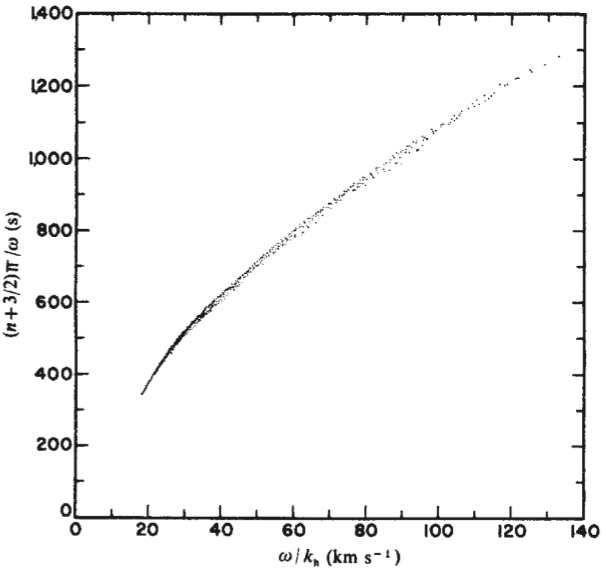
\includegraphics[keepaspectratio,width=0.4\textwidth]{dispersionDuvall}
\caption{Inversione del profilo radiale della velocit\'a del suono tramite inversione di \refeq{eq:analinversionc}: linea continua. La linea tratteggiata \'e la velocit\'a del suono calcolata sulla base di un modello solare. Da \cite{christensen1985speed}.}
\end{wrapfigure}

Determinando sperimentalmente $F(\frac{\omega}{L})=F(w)$ l'equazione \eqref{eq:duvallf} pu\'o essere invertita analiticamente

\begin{equation}
r=R\Exp{-\frac{2}{\pi}\int_{a_s}^a(w\expy{-2}-a\expy{-2})\expy{-\frac{1}{2}}\TDy{w}{F}\,dw}\label{eq:analinversionc}
\end{equation}

dove $a=\frac{c_s}{r}$.

\subsection{Struttura dei modi penetranti nel core stellare}

Per modi di basso grado \'e possibile usare l'espressione \eqref{eq:freqequi} che riscrive la legge di Duvall come
\begin{equation}\label{eq:claverie}
    \nu_{nl}=\frac{\omega_{nl}}{2\pi}\approx(n+\frac{l}{2}+\frac{1}{4}+\alpha)\Delta\nu
\end{equation}
con $\Delta\nu=[\int_0^R\frac{dr}{c_s}]\expy{-1}$.

La deviazione dalla \eqref{eq:claverie} fornisce informazioni sull'evoluzione chimica del core di fusione: infatti estendendo ancora l'espansione di \eqref{eq:duvallf} si ha una misura della variazione di $c$ nel core della stella
\begin{equation}\label{eq:tassoul}
    d_{nl}=\nu_{nl}-\nu_{n-1,l+2}\approx-(4l+6)\frac{\Delta\nu}{4\pi^2\nu_{nl}}\int_0^R\frac{dc_s}{dr}\frac{dr}{r}
\end{equation}
La velocit\'a del suono \'e ridotta a causa dell'aumentare di $\mu$ durante la fusione di H in He durante l'evoluzione stellare: il centro solare \'e un minimo locale per la velocit\'a del suono e quindi, essendo il gradiente della velocit\'a del suono positivo, la parte centrale da un contributo sempre pi\'u negativo in \eqref{eq:tassoul} con l'evolversi della stella.

\subsection{Duvall linearizzata}

Introducendo nella relazione di Duvall \eqref{eq:duvallexpli} le differenze tra le grandezze relative a due modelli solari o modello solare e frequenze osservate ottengo
\begin{equation}
S_{nl}\frac{\delta\omega_{nl}}{\omega_{nl}}\approx H_1(\frac{\omega_{nl}}{L})+H_2(\omega_{nl}),\ S_{nl}=\int_{r_t}^R(1-\frac{L^2c^2}{r^2\omega_{nl}^2})\expy{-\frac{1}{2}}\frac{dr}{c}-\pi\TDy{\omega}{\alpha}
\end{equation}
dove ho definito
\begin{equation}
H_1(w)=\int_{r_t}^R(1-\frac{c^2}{r^2w^2})\expy{-\frac{1}{2}}\frac{\delta_rc}{c}\frac{dr}{c},\ H_2(\omega)=\frac{\pi}{\omega}\delta\alpha(\omega)
\end{equation}
ottenute separatamente attraverso fitting dei dati sperimentali e contenenti la prima il contributo alle differenze nelle frequenze dei modi dovuto alle differenze del profilo radiale della velocit\'a del suono, la seconda alle diffenze nella regione vicino alla superficie.

Dalla rozza approssimazione $\frac{\delta\omega}{\omega}\approx\frac{\int_{r_t}^{R}\frac{\delta_rc_s}{c_s}\frac{dr}{c_s}}{\int_{r_t}^R\frac{dr}{c_s}}$ si vede che le differenze nella velocit\'a del suono nelle varie regioni influiscono sulle differenze nelle frequenze con un peso dato dal tempo impiegato da un'onda sonora ad attraversare la regione: le differenze nella regione vicino alla superficie dove $c_s$ \'e minore hanno un effetto relativamente grande sulle differenze di frequenza.

Una volta determinato $H_1$ le differenze nel profilo radiale di $c_s$ sono determinate tramite
\begin{equation}
\frac{\delta_rc_s}{c_s}=-\frac{2a}{\pi}\TDof{\ln{r}}\int_{a_s}^a(a^2-w^2)\expy{-\frac{1}{2}}H_1(w)\,dw
\end{equation}

%buon accordo range $0.2-095\ \rsun{}$.
%Le differenze in $c_s$ corrispondono a errori nel modello in $\frac{T}{\mu}$ minori del $2\%$.
%confronto diffusion no diffusion model.
%separation opacity uncertainties from effects of diffusion and settling.
%Inversione di $H_2$ ?? H He ionization zones.

La funzione $H_2$ \'e determinata dalla regione sotto la fotosfera. \cite{chr92phase}, analizzando la relazione tra $H_2(\omega)$ e le differenze in $c_s(r)$ e $\Gamma_1$ nelle regioni esterne, hanno visto che discrepanze pi\'u vicino alla superficie generano una componente lentamente oscillante in $H_2(\omega)$ e la ''frequenza'' aumenta con l'aumentare della profondit\'a. \'E inoltre possibile indagare l'andamento di $\Gamma_1$ nella regione di seconda ionizzazione di He e pi\'u in generale il comportamento di $H_2(\omega)$ nelle zone di ionizzazione di H e He consente un'analisi dell'equazione di stato e determinazione dell'abbondanza di elio nella zona convettiva.

% Dalsnotes 7.155, fig 7.15
%vedi relative sharp variations in $\Gamma_1$ in He second ionization zone Influence of the upper layers of the sun on the p-mode frequencies

{\let\clearpage\relax\let\cleardoublepage\relax \chapter{Inversione non asintotica.}} % Inizio chapter "Inversione non asintotica." senza nuava pagina

La soluzione del problema inverso per il sistema completo di equazioni si basa sulla linearizzazione delle variazioni attorno ad un modello di cui siano calcolabili le autofunzioni del vettore moto perturbato $\vec{\xi}$: il problema \'e espresso matematicamente da \eqref{eq:variational}. Faccio l'esempio della correzione alle frequenze dei modi causata dalla rotazione.

%Asymptotic approximation for radial eigenfunction (integral equation connectin sound speed $c(r)$ to $\Omega_{nl}$) is inadequate (especially in deep interior)

\section{Principio variazionale}    %Vedi pg 110 dalsnote.

Riscrivo l'equazione del moto linearizzata \eqref{eq:emper} nella forma
\begin{equation}
-\omega^2\Lvar{\vec{r}}=\frac{1}{\rho}\nabla p'-\vec{g}'-\frac{\rho'}{\rho}\vec{g}=L(\Lvar{\vec{r}})\label{eq:eigenhermitian}
\end{equation}
\citet{Cha64Variational} ha dimostrato che questo costituisce un problema agli autovalori hermitiano per condizioni ai bordi di pressione e densit\'a nulle.

Non essendo possibile misurare le autofunzioni delle oscillazioni lineari adiabatiche per l'interno solare si linearizza il problema attorno ad un modello solare per cui siano calcolabili mentre  le oscillazioni di un altro modello o del Sole stesso sono descritte da 
\begin{equation}
(L+\Lvar{L})(\xi+\Lvar{\xi})=-(\omega+\Lvar{\omega})^2(\xi+\Lvar{\xi}) 
\end{equation}
quindi la variazione delle frequenze \'e determinata da 

\begin{equation}\label{eq:variational}
\frac{\Lvar{\omega}}{\omega}=-\frac{\int_V\rho\vec{\xi}\Lvar{L}\vec{\xi}\,d^3x}{2\omega^2\int_V\rho\scap{\xi}{\xi}d^3x}
\end{equation}
dove $\vec{\xi}=\Lvar{\vec{r}}$ \'e autovettore (perturbazione lagrangiana) del problema agli autovalori \eqref{eq:eigenhermitian}.

\section{Rotazione.}

[Inversione 2d vs 1.5d]
[Kernel rotazione e risoluzione: \cite{}]
[Completare relazioni splitting inversione 1.5d]


Il Sole \'e un rotatore lento: le osservazioni della superficie mostrano una dipendenza dalla co-latitudine 
\begin{equation*}
\frac{\Omega(\theta)}{2\pi}=\SI{451.5}{\nano\hertz}-\SI{65.3}{\nano\hertz}\cos^2{\theta}-\SI{66.7}{\nano\hertz}\cos^4{\theta}
\end{equation*}
questa legge soggetta a discrepanze e variazioni temporali.

\begin{figure}[!h]
\centering
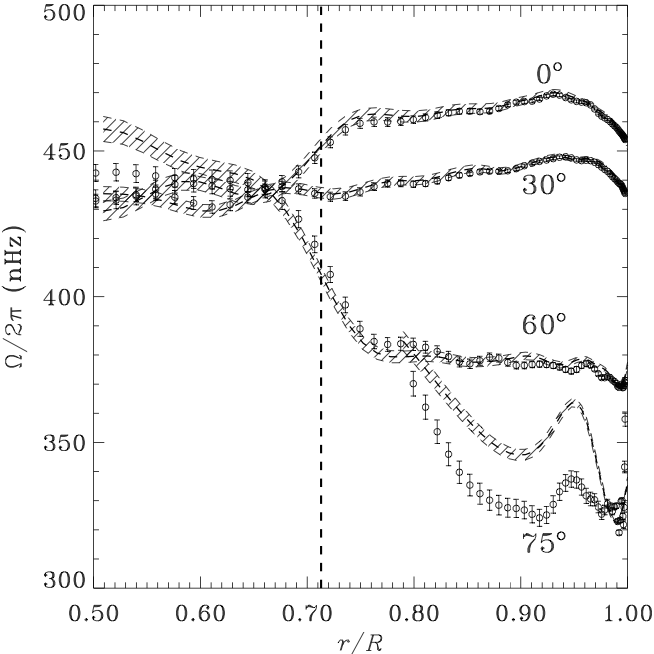
\includegraphics[keepaspectratio,width=0.8\textwidth]{invertedrotation}
\caption{Inversione della velocit\'a di rotazione a diverse latitudini. La linea verticale tratteggiata indica la base della zona convettiva. Da \cite{chr02helioseismology}.}
\end{figure}

Considero la correzione al primo ordine in $\Omega$. Il campo di velocit\'a rotazionale in coordinate sferiche \'e 
\begin{align}
&\vec{v_0}=(0,0,r\Omega\sin{\theta})=\vecp{\Omega}{r}\\
&\vec{\Omega(r,\theta)}=(\Omega(r,\theta)\cos{\theta},-\Omega(r,\theta)\sin{\theta},0)
\end{align}

In assenza di moti macroscopici il termine d'inerzia \'e $\rho_0\TDy{t}{\vec{v}}=\rho_0\PtwoDy{t}{\vec{\xi}}$, mentre in caso di rotazione si ha
\begin{equation}
\rho_0(\PDof{t}+\scap{v_0}{\nabla})^2\vec{\xi}
\end{equation}

Considero il termine dovuto alla rotazione come una piccola correzione alle frequenze dei modi
\begin{align}
&\omega_{(l,m)}+\Delta\omega_{(l,m)}&\intertext{quindi l'equazione del moto al primo ordine nella perturbazione, con $\alpha=(l,m)$, \'e}\nonumber\\
&\rho_0(\omega_{\alpha}^2+2\omega_{\alpha}\Delta\omega_{\alpha})\vec{\xi}=\nabla P_1-\frac{\rho_1}{\rho_0}\nabla P_0+\rho_0\nabla\Phi_1+2i\omega_{\alpha}\rho_0(\scap{v_0}{\nabla})\vec{\xi}\\
&\intertext{da cui si deduce}\nonumber\\
&\Delta\omega_{\alpha}=\frac{i\int\rho_0\xi_{\alpha}^*(\scap{v_0}{\nabla})\xi_{\alpha}}{\int\rho_0\xi_{\alpha}^*\xi_{\alpha}}=\frac{-m\int\rho_0\Omega\xi_{\alpha}^*\xi_{\alpha}\,dV+i\int\rho_0\xi_{\alpha}^*(\vecp{\Omega}{\xi_{\alpha}})\,dV}{\int\rho_0\xi_{\alpha}^*\xi_{\alpha}}
\end{align}

Il problema di trovare $\Omega(r,\theta)$ dalla differenza $\Delta\omega_{\alpha}$ \'e lineare in $\Omega$ quindi $\Delta\omega_{\alpha}\propto\Omega$. Per determinare quindi la rotazione dobbiamo conoscere l'autovalore $\xi_{\alpha}$ dello stato imperturbato.

%Per rotazione puramente radiale $\Omega(r)$ la relazione tra lo splitting delle frequenze e la rotazione \'e
%\begin{equation}
%\Delta\omega_{\alpha}=-m\frac{\int_0^{\rsun{}}\rho_0\Omega\{|\xi_r-\xi_h|^2+[l(l+1)-2]|\xi_h|^2\}r^2\,dr}{\int_0^{\rsun{}}\rho_0\{|\xi_r|^2+l(l+1)|\xi_h|^2\}r^2\,dr}=\int_0^{\rsun{}}K_{\alpha}(r)\Omega(r)\,dr
%\end{equation}
%Any given $\Delta\omega_{\alpha}$ samples angular velocity in the depth range corresponding to $\xi_{\alpha}$.

La velocit\'a angolare contribuisce a $\Delta\omega_{\alpha}$ negli strati in cui $\xi_{\alpha}$ \'e apprezzabile. Nel caso di rotazione dipendente solo da r si ha che $\Delta\omega_{\alpha}$ \'e lineare in m: ho $2l+1$ frequenze equispaziate.

%Per investigare la dipendenza $\Omega(r,\theta)$ devo considerare le $2l+1$ frequenze.
%latitudinal shear causa una deviazione da frequenze equispaziate.

%% corretto fin qui

\section{Correzioni struttura idrostatica.}

Utilizzo le equazioni che descrivono le oscillazioni adiabatiche \eqref{eq:contper}, \eqref{eq:emper}, \eqref{eq:adper}, \eqref{eq:gapert} per scrivre l'equazione del moto variazionale nella forma
\begin{equation}
\Lvar{L}\vec{\xi}=\nabla(\Lvar{c^2}\nabla\cdot\vec{\xi}+\Lvar{\vec{g}}\cdot\vec{
\xi})+\nabla(\frac{\Lvar{\rho}}{\rho})c^2\nabla\cdot\vec{\xi}+\frac{1}
{\rho}\nabla\rho\Lvar{c^2}\nabla\vec{\xi}+\Lvar{\vec{g}}\nabla\cdot\vec{\xi}-
G\nabla\int_V\frac{\nabla\cdot(\Lvar{\rho}\xi)}{|\vec{x}-
\vec{x}'|}\,d^3x'\label{eq:eqmotvar}
\end{equation}
con
\begin{equation}
\Lvar{g}(r)=\frac{4\pi G}{r^2}\int_0^r\Lvar{\rho}(s)s^2\,ds
\end{equation}

Determino le differenze tra le frequenze osservate e quelle relative ad un modello, $\delta\omega_{nl}=\Omega_{\odot}-\Omega_{Mod}$, e le differenze nella stratificazione idrostatica tramite l'inversione per le variabili $(\rho,c^2)$

\begin{align}
&\frac{\delta\omega_{nl}}{\omega_{nl}}=\int_0^R[K^{nl}_{c^2,\rho}(r)\frac{\delta_rc^2}{c^2}(r)+K^{nl}_{\rho,c^2}(r)\frac{\delta_r\rho}{\rho}(r)]\,dr+I_{nl}\expy{-1}F_{Surf}(\omega_{nl})+\sigma_i\label{eq:invstructure}&\intertext{dove $\sigma_i$ \'e l'incertezza sulle frequenze osservate e}\nonumber\\
&\frac{\delta_rc^2}{c^2}(r)=\frac{[c_{\odot}^2(r)-c_{mod}^2(r)]}{c^2(r)},\ \frac{\delta_r\rho}{\rho}(r)=\frac{[\rho_{\odot}(r)-\rho_{mod}(r)]}{\rho(r)}
\end{align}

I kernel $K_Q^j$ dipendono dalle autofunzioni del modello, il termine $E_{nl}\expy{-1}F_{Surf}(\omega_{nl})$, con $E_{nl}=\int_V|\Lvar{\vec{r}}|^2\rho\,dV$, \'e una correzione dovuta alle differenti condizioni fisiche che si incontrano vicino alla superficie: i modi con basse frequenze sono riflessi pi\'u in profondit\'a a $\omega=\omega_c$ e quindi sono meno influenzati dagli strati superficiali.

Esplicito la relazione linearizzata tra le differenze nelle grandezze $\rho$, g, P, $c^2$ e le differenze nelle frequenze sostituendo \eqref{eq:eqmotvar} in \eqref{eq:variational}:
\begin{align}
&F_{Surf}(\omega)-\frac{1}{2\omega^2}(I_1+I_2+I_3+I_4)=E_{nl}\frac{\Lvar{\omega}}{\omega}&\intertext{con}\nonumber\\
&I_1=-\int_0^R\rho(\scap{\nabla}{\xi})^2\Lvar{c^2}r^2\,dr\\
&I_2=\int_0^R\xi_r[\rho\scap{\nabla}{\xi}+\nabla\cdot(\rho\vec{\xi})]\Lvar{g}r^2\,dr\\
&I_3=\int_0^R\rho c^2\xi_r\scap{\nabla}{\xi}\PDof{r}(\frac{\Lvar{\rho}}{\rho})r^2\,dr\\
\begin{split}
&I_4=\frac{4\pi G}{2l+1}\int_0^R\divof{}(\rho\vec{\xi})r^2\,dr[\frac{1}{r\expy{l+1}}\int_0^rs\expy{l+2}(\rho\divec{\xi}-\rho\TDy{s}{\xi_r}-\frac{l+2}{s}\rho\xi_r)\frac{\Lvar{\rho}}{\rho}\,ds\\
&+r^l\int_r^R\frac{1}{s\expy{l-1}}(\rho\divec{\xi}-\rho\TDy{s}{\xi_r}-\frac{1-l}{s}\rho\xi_r)\frac{\Lvar{\rho}}{\rho}\,ds]
\end{split}
\end{align}

Per distinguere gli effetti dovuti alla non corretta descrizione fisica dei modi vicino alla superficie, $r>0.95\rsun{}$, cui sono pi\'u sensibili i modi di l elevato, si introduce
\begin{equation}
Q_{nl}=\frac{E_{nl}}{E^0_{nl}}\label{eq:surfaceeffects}
\end{equation}
che vale 1 per $l=0$ e diminuisce al crescere di $l$.

%[figura dalsgaard 2002 fig deltanu/deltanu]
%Nel caso l'entit\'a delle correzioni a $\rho$ e $c^2$ non giustifichi l'approssimazione lineare si ha un miglior accordo definendo la differenza tramite $\frac{\Lvar{f}}{f}=\frac{f-f_0}{\sqrt{ff_0}}$.

Le correzioni alle pressione si ottengono dall'equazione di equilibrio idrostatico \eqref{eq:fidroequilibrio}
\begin{equation}
\Lvar{P}=\int_r^R(g\Lvar{\rho}+\rho\Lvar{g})\,dr\label{eq:pressurecorrho}
\end{equation}

%% discrepanza densita e velocita suono con metallicita riviste
%[figure inversione al variare dei parametri solari da \cite{boothroyd2003our}]

[reminder: errori: sperimentali/numerici/modello per inversione $(\rho,c^2)$]
\begin{wraptable}{r}{5.5cm}
\begin{tabular}{||}
&\Delta_{exp}&\Delta_{num}&\Delta_{mod}\\
\frac{\delta c}{c}&0.02\percent&&\\
\frac{\delta\rho}{\rho}&\\
\end{tabular}
\end{wraptable}

\subsection{Inversione equazione di stato e composizione.}

Per investigare la composizione \'e necessario usare l'equazione di stato per esplicitare $\Gamma_1(P,\rho,X_i)$ riscrivendo \eqref{eq:variational} nella forma

\begin{align}
&\frac{\delta\omega_{nl}}{\omega_{nl}}=\int_0^R[K^{nl}_{\Gamma_1,\rho}(r)\frac{\delta_r\Gamma_1}{\Gamma_1}(r)+K^{nl}_{\rho,\Gamma_1}(r)\frac{\delta_r\rho}{\rho}(r)]\,dr+I_{nl}\expy{-1}F_{Surf}(\omega_{nl})+\sigma_i\label{eq:invdGammadrho}&\intertext{da questa, utilizzando l'equazione di stato per ricavare la dipendenza di $\Gamma_1$ dalla composizione chimica, \'e possibile ottenere il profilo radiale di $Y$: per diminuire gli errori sistematici dovuti alle discrepanze nell'equazione di stato e nella metallicit\'a riscrivo l'ultima espressione nella forma:}\nonumber\\
&\frac{\delta\omega_{nl}}{\omega_{nl}}=\int_0^RK^{nl}_{u,Y}(r)\frac{\delta_ru}{u}(r)\,dr+\int K^{nl}_{Y,u}(r)\delta_rY\,dr+\int_0^RK^{nl}_{c^2,\rho}(r)(\frac{\delta\Gamma_1}{\Gamma_1})_{int}\,dr+I_{nl}\expy{-1}F_{Surf}(\omega_{nl})\label{eq:diffthermo}&\intertext{dove $(\delta\Gamma_1)_{int}$ \'e l'errore dovuto alle discrepanze nell'equazione di stato a $(P,\rho,Y)$ fissati.}\nonumber
\end{align}
La determinazione dell'abbondanza di elio nella regione convettiva \'e dovuta principalmente alla deviazione da $\Gamma_1=\frac{5}{3}$ nella regione di seconda ionizzazione dell'elio.

%Esprimendo $\delta_rc^2$ in termini di $\delta_ru=\delta_r(\frac{P}{\rho})$, $\delta_rY$ e $\delta_r\Gamma_1$, riscriviamo \eqref{eq:invstructure}, dove abbiamo utilizzato l'equazione di stato per descrivere la dipendenza di $\Gamma_1$ dall'abbondanza di $\cel{He}{4}{}{}$:
% Dals Art pg 31-32
%Le differenze in $U$ e $\rho$  fra modelli solari sismologici e modelli solari standard sono al massimo pochi per cento.

[reminder: EOS dependence:LInantiabasu07]
[reminder: errori: sperimentali/numerici/modello per inversione $(\rho,Y)$, $(\rho,\Gamma_1)$]

\section{Tecniche di inversione numeriche.}
%vedi JCD 2002 pg 25-32

Elenco alcune tecniche numeriche usate.

I risultati dell'inversione sono affetti da errori sistematici introdotti dalla procedura di inversione ([vedi effetti risoluzione finita sunto pg 1098 $\S 10$ pbp 2000 e DDFR97]).

\subsection{Minimi quadrati}

Si parametrizzano le funzioni incognite $\frac{\delta_rc^2}{c^2}$, $\frac{\delta_r\rho}{\rho}$, $F_{Surf}$. Attraverso la tecnica dei minimi quadrati si ottengono i parametri e le correzioni. La funzione da minimizzare \'e
\begin{align}
&Y=(N-N_p)\chi^2+\alpha N\int_0^1(x\TDof{x}\frac{\Delta u}{u})^2\,dx\label{minimizerls}&\intertext{con}\nonumber\\
&\chi^2=\frac{1}{N-N_p}\sum_{\alpha=1}^N(\frac{\Delta\nu_{obs}-\Delta\nu_{fit}}{\sigma})^2_{\alpha}
\end{align}
N indica il numero totale di modi $\alpha$, $N_p$ il numero di parametri da determinare, $\Delta\nu_{fit}$ contiene le funzioni incognite opportunamente parametrizzate ed \'e dato da \eqref{eq:diffthermo} o \eqref{eq:invstructure}, $\sigma$ \'e l'errore osservativo e il secondo addendo del lato destro di \eqref{eq:minimizerls} \'e introdotto per ridurre oscillazioni indesiderate nel risultato dell'inverisone con $\alpha$ parametro di regolarizzazione.

%Determinazione incertezza.
%(Dziembowski90, Antia Basu 94), (JCD90).

\subsection{Subtractive Optimally Localized Averaging}

Per determinare in generale la funzione $\frac{\delta f_1(r)}{f_1(r)}$ scelgo i $c_i(r_0)$ tali che $\sum c_i(r_0)\frac{\delta\omega_i}{\omega_i}$ fornisca una media del valore di $\frac{\delta f_1(r)}{f_1(r)}$ in $r=r_0$:

\begin{align*}
&\sum_ic_i(r_0)\frac{\delta\omega_i}{\omega_i}=\int_0^R\sum_ic_i(r_0)K_{1,2}^i(r)\frac{\delta f_1(r)}{f_1(r)}\,dr+\int_0^R\sum_ic_i(r_0)K_{2,1}^i(r)\frac{\delta f_2(r)}{f_2(r)}\,dr+\sum_ic_i(r_0)\frac{F_{Surf}(\omega_i)}{\omega_i}
\end{align*}

Il primo termine approssima il valore di $\frac{\delta f_1}{f_1}$ pesato dal kernel $\mathcal{K}(r,r_0)=\sum_ic_i(r_0)K_{1,2}^i(r)$, il secondo tiene conto dell'influenza che hanno le discrepanze della seconda funzione su quelle della funzione che abbiamo scelto di invertire pesate da $\mathcal{L}_{21}(r_0,r)=\sum_ic_i(r_0)K_{21}^i(r)$, il terzo \'e il termine di superficie: i coefficienti $c_i(r_0)$ sono scelti in maniera da riprodurre la funzione target, minimizzare la contaminazione delle $\frac{\delta f_2}{f_2}$ via $\mathcal{L}_{21}$ e il rumore.

I parametri si trovano minimizzando
\begin{align*}
&\int(\sum_ic_iK_{12}^i)^2\,dr+\beta\int(\sum_ic_iK_{21}^1)^2\,dr+\mu\sum_{ij}c_ic_jE_{ij}
\end{align*}
$\beta$ \'e un parametro per il contributo del secondo termine, $E$ \'e una matrice che rappresenta le incertezze sulle frequenze osservate.

Illustro la tecnica SOLA per determinare $\frac{\delta_rc^2}{c^2}$: si formano delle combinazioni lineari di $\frac{\Lvar{\omega_i}}{\omega_i}$ pesate da coefficienti $c_i(r_0)$ tali che $\frac{\Lvar{c^2}}{c^2}$ sia centrato attorno $r_0$ e che gli altri termini in \eqref{eq:invstructure} siano soppressi, queste compongo un averaging kernel $\mathcal{K}_{c^2,\rho}(r_0,r)=\sum_ic_i(r_0)K_{c^2,\rho}^i(r)$, con $\int_0^R\mathcal{K}(r_0,r)\,dr$. La natura precisa della localizzazione \'e determinata da una funzione target la cui larghezza \'e anch'essa parametro del fit.


Determino i varii coefficienti minimizzando l'espressione
\begin{align}
&\int_0^R[\mathcal{K}_{c^2,\rho}(r_0,r)-\mathcal{T}(r_0,r)]^2\,dr+\beta\int_0^R\mathcal{G}_{\rho,c^2}(r_0,r)\,dr+\mu\sum_i\sigma_ic_i(r_0)c_j(r_0)\\
&\mathcal{G}_{\rho,c^2}(r_0,r)=\sum_ic_i(r_0)K_{\rho,c^2}^i(r)&\intertext{il kernel cross-term  contralla i contributi indesiderati di $\frac{\delta_r\rho}{\rho}$}\nonumber
\end{align}


{\let\clearpage\relax\let\cleardoublepage\relax
\chapter{Vincoli al modello solare dalle osservazioni sismologiche.}%%chapter: vincoli al modello solare: HCSM.
}


[variazioni in opacit\'a vs variazioni in $\midfrac{Z}{X}$.]
[Dipendenza dell'inversione dal modello di riferimento.]


\section{Modello solare sismologico.}

%Indico con $Q(P)$ e $Q_{\odot}$ i valori di una grandezza Q determinati tramite un modello solare, funzione dei parametri del modello, e risultanti dalle correzioni sismologiche a quest ultimi  
%\begin{equation}
%&Q_{\odot}=Q(P)+q(\omega)
%\end{equation}

\subsection{Zona convettiva}

[accuratezza inversione $R_b$, $Y_{ph}$, $\rho_b$]

\begin{wrapfigure}[]{r}{0.4\textwidth}
\centering
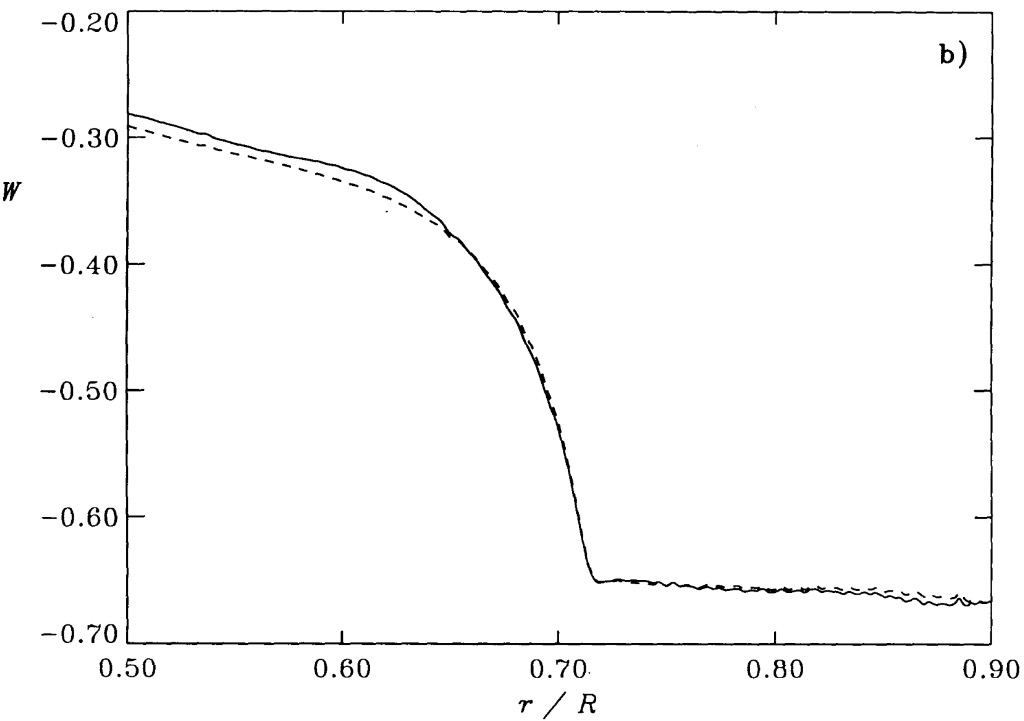
\includegraphics[keepaspectratio,width=0.35\textwidth]{adcsgrad}
\caption{. Da \cite{christensen1991depth}.}
\end{wrapfigure}


Le osservabili sismologiche che caratterizzano la zona convettiva sono $R_b$, $Y_{ph}$ e $c_b$, $\rho_b$.

\begin{itemize}

\item L'abbondanza di elio \'e determinata da varii autori in un range $Y_{ph}=\numrange{0.226}{0.260}$.
%Il valore di $Y_{ph}$ inferiore di \numrange{0.27}{0.28}, richiesto per calibrare i modelli con la luminosit\'a attuale, conferma l'importanza della diffusione dell'elio verso il centro di gravit\'a.
    
\item Profondit\'a della zona convettiva.

La regione radiativa ha stratificazione sub-adiabatica mentre a partire da $r=R_b$ si ha stratificazione quasi-adiabatica,  $\Gamma_1\approx\frac{5}{3}$: $P\propto\rho\expy{\frac{5}{3}}$. Per identificare il raggio a cui si ha il passaggio dal gradiente di temperatura subadiabatico ad adiabatico \'e utile considerare la funzione
\begin{equation}
W=\frac{r^2}{Gm(r)}\TDy{r}{c^2}=\Gamma_1(\invers{\PDly{\rho}{P}}-1)
\end{equation}

    
\begin{align*}
&\frac{R_b}{\rsun{}}=\numrange{0.710}{0.716}\\
&c_b=\SIrange{0.221}{0.225}{\mega\meter\per\second}
\end{align*}

\item Determinati tramite inversione il profilo radiale di u e $R_b$ si determina anche la densit\'a della base della zona convettiva:
\begin{equation*}
\rho_b=\SIrange{0.185}{0.199}{\gram\per\cubic\cm}
\end{equation*}
    
\end{itemize}

[\cite{deg97helioseismology} fig.3]


\subsection{Reazioni nucleari}

%[figure inversione al variare dei parametri solari da \cite{boothroyd2003our}]

\begin{figure}[!h]
\centering

\begin{subfigure}[t]{0.32\textwidth}
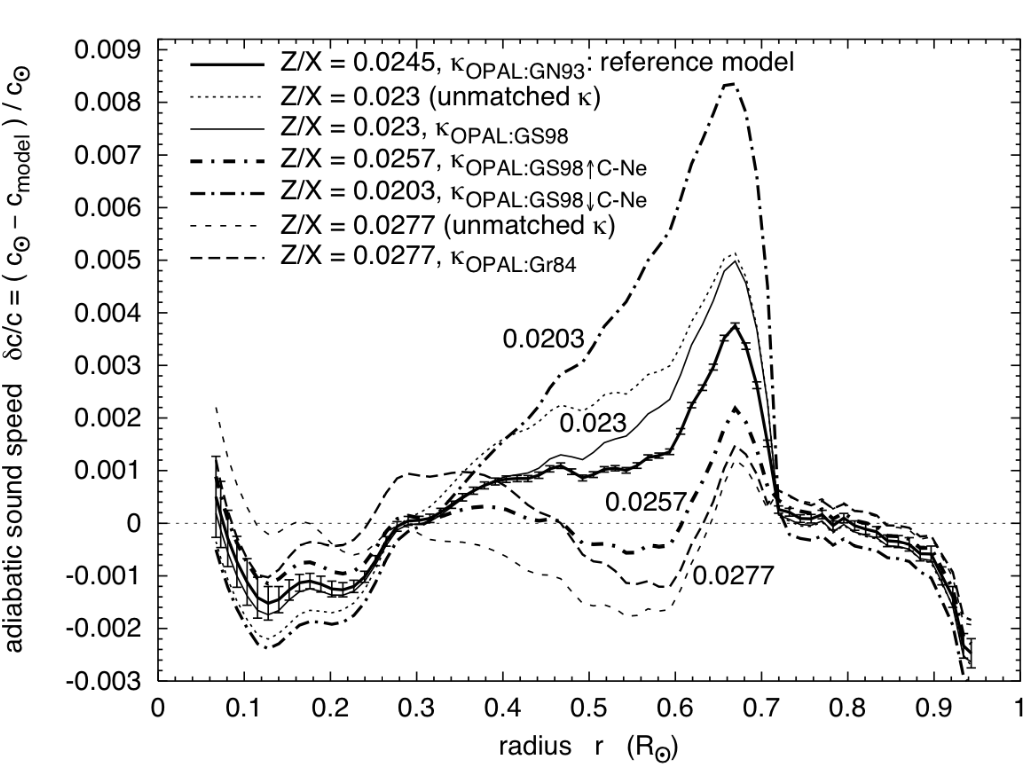
\includegraphics[width=0.99\textwidth,keepaspectratio]{soundinvZ}
\end{subfigure}
~
\begin{subfigure}[t]{0.32\textwidth}
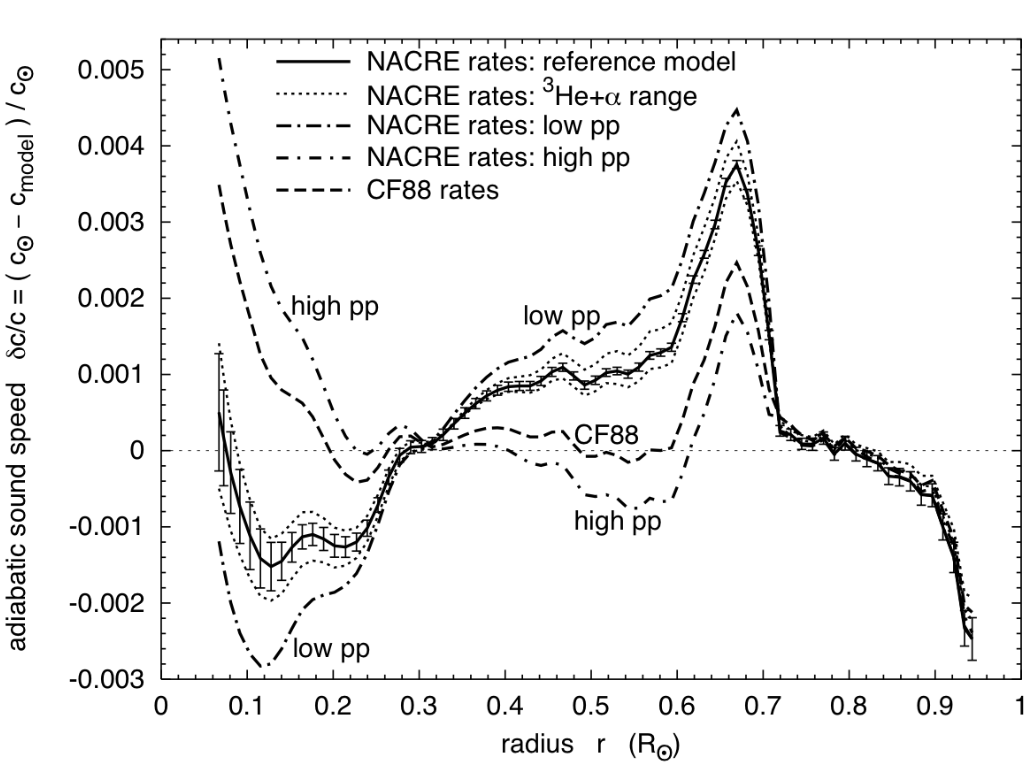
\includegraphics[width=0.99\textwidth,keepaspectratio]{soundinvRR}
\end{subfigure}
~
\begin{subfigure}[t]{0.32\textwidth}
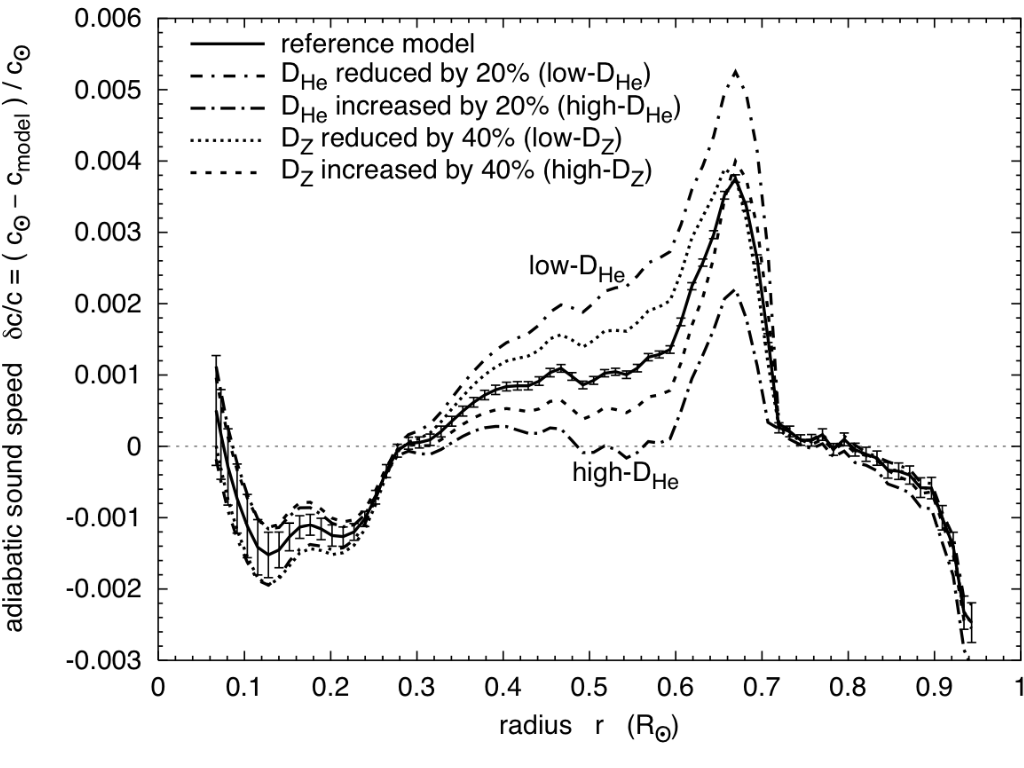
\includegraphics[width=0.99\textwidth,keepaspectratio]{soundinvDiff}
\end{subfigure}
\caption{Da \cite{boothroyd2003our}.}

\end{figure}

\begin{figure}[!h]
\centering
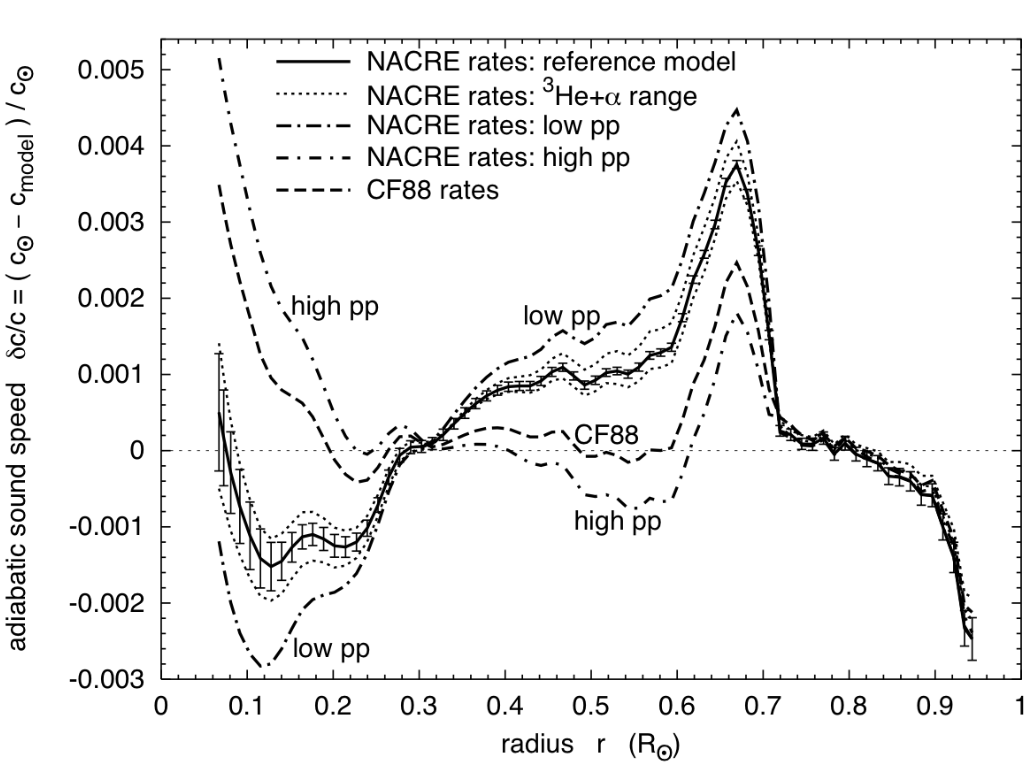
\includegraphics[width=0.99\textwidth,keepaspectratio]{soundinvRR}
\caption{Da \cite{boothroyd2003our}.}
\end{figure}

\section{Approssimazione di scaling.}

Oltre a determinare il valore sismologico corretto delle grandezze meccaniche del modello solare si pu\'o stabilire il range dei parametri del SSM compatibili con le frequenze osservate: si approssima localmente una dipendenza della grandezza $Q$ dai parametri della forma $\frac{Q}{Q_{MSS}}=(\frac{P}{P_{MSS}})\expy{\alpha_{QP}}$ quindi si determina il range dei parametri $p_i=\frac{P^i}{P_{MSS}^i}$ compatibile con $\Omega_i\pm\Delta\Omega_i$, in particolare si usano le grandezze sismologiche pi\'u accurate $Y_{ph},\ R_b,\ \rho_b$.

{Regione intermedia con $0.2<x<0.65$.}

(Vedi: \cite{bah04accurately})
Sotto la zona convettiva $\Gamma_1=\frac{5}{3}$ con accuratezza migliore di \num{e-3}. L'inversione sismologica \'e accurata: $\frac{\Delta u}{u}\leq5 \permil$. Dalla conoscenza di $u_{\odot}$ si ricava il profilo radiale della velocit\'a del suono tramite $c_s^2=\Gamma_1 u$.

% Vedi H,SManf scilla pg 11-12
%Le propriet\'a di questa regione sono determinate dall'opacit\'a e quindi, nella misura in cui \'e possibile combinare le differenze nei modi per cancellare il contributo della zona convettiva e considerare il contributo di $\frac{\Lvar{L}}{L}$ una piccola correzione, come accade fuori dalla regione di produzione di energia, \'e possibile studiare gli effetti delle variazioni di opacit\'a sui modi.
%La quantit\'a da determinare \'e quindi
%\begin{equation}
%\frac{\delta\kappa}{\kappa}=\frac{\Lvar{\kappa}}{\kappa}+\Dcvar{\PDly{\rho}{\kappa}}{T}+\frac{\Lvar{T}}{T}\Dcvar{\PDly{T}{\kappa}}{\rho}
%\end{equation}
%dove $\frac{\Delta\kappa}{\kappa}$ rappresenta la correzione a $\kappa(\rho,T)$ a densit\'a, temperatura e composizione fissate.
[vedi fig 11/12 \cite{ell95opacity} ??]


{Core di fusione $x<0.2$.}

Vedi \cite{ell98relativistic}

%Inversione di $(\delta\Gamma_1)_{int}$ mostra la necessit\'a di tener conto degli effetti relativistici per gli elettroni, che nel core solare hanno energia termica \SI{1.35}{\kilo\ev} approx $0.3\%$ of $m_e$).

\begin{align}
&\frac{\Lvar{\Gamma_1}}{\Gamma_1}\approx-\frac{2+2X}{3+5X}T&\intertext{dove T \'e in unit\'a di $\frac{m_ec^2}{k}$}\nonumber
\end{align}

%[\cite{ell98relativistic} fig.3 ].
%[Solar neutrino deduced from solar seismic model]

La temperatura centrale dipende principalmente dall'opacit\'a e dal rapporto $\frac{Z}{X}$. Nella regione centrale si determina
\begin{align}
&R_b=R_{b,MSS}z\expy{-0.046}k\expy{-0.0084}\\
&\rho_b=\rho_{b,MSS}z\expy{0.47}k\expy{0.095}\\
&Y_{ph}=Y_{ph,MSS}z\expy{0.31}k\expy{0.61}&\intertext{dove k e z si riferiscono a opacit\'a e rapporto metalli/idrogeno.}\nonumber
\end{align}

Il valore ottimale dei parametri $(k,z)$ si determina minimizzando
\begin{equation}
\chi^2(z,k)=\sum_i(\frac{Q_{\odot i}-Q_i(z,k)}{\Delta Q_i})^2
\end{equation}
quindi per la temperatura centrale del Sole si ha 
\begin{equation}
T_{ES}=T_{MSS}(\frac{Y_{ph\odot}}{Y_{ph,MSS}})\expy{0.2}=\SI{1.587e7}{\kelvin}
\end{equation}


\end{document}